\documentclass[12pt, letterpaper, fleqn]{article}
\usepackage[letterpaper, margin=.75in]{geometry}
\usepackage[utf8]{inputenc}
\usepackage{amsmath}
\usepackage{amssymb}
\usepackage{algorithmicx}
\usepackage{algpseudocode}
\usepackage{algorithm}
\usepackage[english]{babel}
\usepackage{amsthm}
\usepackage{graphicx}
\usepackage{xcolor}
\graphicspath{ {.} }
\usepackage{fancyhdr}
\usepackage{tikz}
\usepackage{hyperref}
\usepackage{cancel}
\newcommand*\circled[1]{\tikz[baseline=(char.base)]{
            \node[shape=circle,draw,inner sep=2pt] (char) {#1};}}
\setlength\parindent{0pt}
\def\join{\mathbin{\ojoin\mkern0mu\bowtie\mkern3mu\ojoin}}

%\pagestyle{fancy}
%\fancyhf{}
%\rhead{Bill Yang}
%\renewcommand{\headrulewidth}{0pt}

\newcommand{\handout}[5]{
   \renewcommand{\thepage}{#1-\arabic{page}}
   \noindent
   \begin{center}
   \framebox{
      \vbox{
%    \hbox to 5.78in { {\bf M328K Number Theory} \hfill #2 }
%       \vspace{4mm}
%       \hbox to 5.78in { {\Large \hfill #5  \hfill} }
%       \vspace{2mm}
%       \hbox to 5.78in { {\it #3 \hfill #4} }
    \hbox to 5.78in { { Bill Yang} \hfill {Due: #2} }
       \vspace{4mm}
       \hbox to 5.78in { {\Large \hfill #5  \hfill} }
       \vspace{2mm}
       \hbox to 5.78in { {#3 \hfill #4} }
      }
   }
   \end{center}
   \vspace*{4mm}
}

\newcommand{\ho}[5]{\handout{#1}{#2}{#3}{Instructor: #4}{Homework #1}}

\begin{document}
  \ho{11}{5/8/20}{CS386D Database Systems}{Daniel Miranker} \\

  \section{Part 1}
  \textbf{1} \\
  a) Openlate(r) $<-$ Restaurant(r, d1, \_, c1) AND Restaurant(r, d2, \_, c2) 
  AND d1 = Friday AND d2 = Saturday AND c1 $>$ 9:00PM AND c2 $>$ 9:00PM \\

  b) Openearly(r) $<-$ Restaurant(r, d1, o1) AND Restaurant(r, d2, o2)
  AND d1 = Saturday AND d2 = Sunday ANd o1 $<$ 8:00AM ANd o2 $<$ 8:00AM\\

  Happyhawk(p) $<-$ Nighthawks(p, r1) AND Nighthawks(p, r2) AND Openlate(r1) AND
  Openearly(r2) \\

  \textbf{2}\\ 
  a) \\
  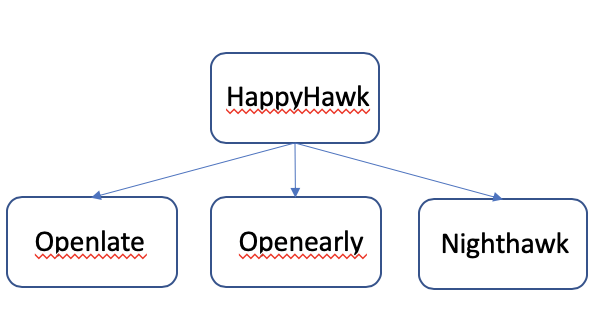
\includegraphics[scale=0.5]{images/depgraph.png} \\
  b) No \\
  c) Before: HappyHawk$(\{\})$,\\
  OpenLate$(\{$Unos 360$\})$,\\
  OpenEarly$(\{\})$, \\
  Nighthawks$(\{($Dan, UNOs 360$), ($Tom, UNOs 360$), ($Tom,
  Magnolia Cafe$)\})$ \\

  After: HappyHawk$(\{$ Tom $\})$ \\
  OpenLate$(\{$Unos 360$, $Magnolia Cafe$\})$,\\
  OpenEarly$(\{$Magnolia Cafe$\})$, \\
  Nighthawks$(\{($Dan, UNOs 360$), ($Tom, UNOs 360$), ($Tom,
  Magnolia Cafe$)\})$ \\
  

  \textbf{3} \\
\begin{tabular} { c | c }
  Fenves  & Goldbart \\
  Fenves & Wood \\
  Goldbart & Fussell \\
  Goldbart & Beckner \\
  Wood & Tewfik \\
  Fussell & Miranker \\
  Fussell & Mok \\
  Beckner & Alcook \\
  Tewfik & Ghosh 
\end{tabular} 
\begin{tabular} { c | c }
  Fenves  & Goldbart \\
  Fenves & Wood \\
  Goldbart & Fussell \\
  Goldbart & Beckner \\
  Wood & Tewfik \\
  Fussell & Miranker \\
  Fussell & Mok \\
  Beckner & Alcook \\
  Tewfik & Ghosh  \\

  Fenves  & Fussell \\
  Fenves  & Beckner \\
  Fenves & Tewfik \\
  Goldbart & Miranker \\
  Goldbart & Mok \\
  Goldbart & Alcook \\
  Wood & Ghosh \\
\end{tabular} 
\begin{tabular} { c | c }
  Fenves  & Goldbart \\
  Fenves & Wood \\
  Goldbart & Fussell \\
  Goldbart & Beckner \\
  Wood & Tewfik \\
  Fussell & Miranker \\
  Fussell & Mok \\
  Beckner & Alcook \\
  Tewfik & Ghosh  \\

  Fenves  & Fussell \\
  Fenves  & Beckner \\
  Fenves & Tewfik \\
  Goldbart & Miranker \\
  Goldbart & Mok \\
  Goldbart & Alcook \\
  Wood & Ghosh \\
  
  Fenves & Miranker \\
  Fenves & Mok \\
  Fenves & Alcook \\
  Fenves & Ghosh \\
\end{tabular} 

  \section{Part 2} 
  \textbf{17.4.1} \\
  A = 5, B = 10 \\
  a) $A := A+B; B := A+B; \\
  $$<$Start $T>$ $<T,A,5,15>$ $<T,B,10,25>$ $<$Commit $T>$ \\
  b) $B:=A+B; A:=A+B$\\
  $<$Start $T>$ $<T,B,10,15>$ $<T,A,5,20>$ $<$Commit $T>$ \\
  c) $A:=B+1; B:=A+1$\\
  $<$Start $T>$ $<T,A,5,11>$ $<T,B,10,12>$ $<$Commit $T>$ \\


  \textbf{17.4.3 b, d} \\
  b) Undo transaction T by writing or making sure that $C=30$, $A=10$ on disk in
  that order.
  Add to log $<T$, abort$>$. \\
  Redo transaction U by writing or making sure that $B=21$, $D=41$ on disk in
  that order. \\
  d) Redo transaction T and U by writing or making sure that $A=11$, $B=21$,
  $C=30$, $D=41$, $E=51$ on
  disk in that order. \\

  \textbf{17.4.4} per 17.4.3 b only \\ 
  b) U has been committed. By undo/redo-logs, values can be written to disk
  before or after the commit happens, thus all values changed by U may or may
  not appear on disk. $B=20$ or $21$, $D=40$ or $41$.\\
  T has not been committed. Technically since a value can be written to disk
  before or after a commit, and can only be written as long as its log has been
  recorded, $A=10$ or $11$, $C=30$ or $31$, $E=50$. E does not have a log entry,
  so it could not have been changed. A very proactive manager may have already
  written A and C, but it is possible that they were not yet. We would not know
  without understanding the crash manager. \\
  

  \textbf{18.1.1 a, b, c} \\
  $r(A);r(B);w(B);r(C);w(C);r(D);w(D);r(E);w(E);$\\

  \textbf{18.2.4 a, b, d} \\
  a) i. $2 < 1$, $3 < 2$ \\
  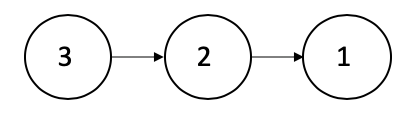
\includegraphics[scale=0.5]{images/agraph.png} \\
  ii. Yes, $T_3, T_2, T_1$\\
  iii. No \\
  b) i. $1<2$, $2<3$, $1<3$ \\
  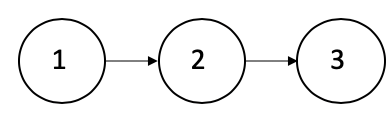
\includegraphics[scale=0.5]{images/bgraph.png} \\
  ii. Yes, $T_1, T_2, T_3$\\
  iii. No \\
  d) i. $1 < 2$, $2<1$\\
  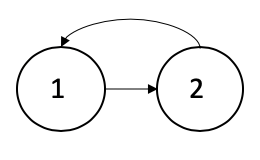
\includegraphics[scale=0.5]{images/dgraph.png} \\
  ii. No \\
  iii. No \\


  \textbf{18.3.3} per b and d \\
  b) The locking scheduler would keep the schedule as it is. No element is
  accessed twice in the same transaction so the lock is locked and unlocked
  immediately every action.\\
  d) $w_2(B)$ would get delayed until $r_1(B)$ executes and unlocks the lock.
  The new schedule would be (without the locks and unlocks): \\
  $r_1(A); r_2(A); w_1(B); r_1(B); w_2(B);r_2(B); w_2(C); w_1(D);$

 
\end{document}
